%\newpage
  \begin{titlepage}
    \vspace*{\fill}
      \part{Evaluation}
    \vspace*{\fill}
  \end{titlepage}

\startcontents[parts]
  
\phantomsection
\chapter*{Contents}

\textit{This part shows the results obtained and the issues that this Facial Expression Recognition system has met. Chapter~\ref{chap:eval_results} gives the results that the system gets and explained them. In Chapter~\ref{chap:eval_issues}, the problems faced are detailed. These issues are mainly concerning \textit{feature extraction} and \textit{real-time}.}

\vspace{\baselineskip}

\printcontents[parts]{}{-1}{\setcounter{tocdepth}{1}}

\pagebreak

\phantomsection
\chapter{Results}
\label{chap:eval_results}

\noindent Two kinds of results have been obtained. First results have been obtained by extracting a test set from the KDEF database, and test it against other subjects from the database. Feature extraction is done by LBP, followed by classification using SVM. The second set of results is obtained with the Kinect in real-time conditions, while the entire KDEF database is used for training. The Kinect gets video sequences of a subject in front of it, his or her face being extracted from these sequences using Viola-Jones algorithm. Then the same feature extraction and classification process is applied to these images.
\newline

\phantomsection
\section{First result set}

\vspace{\baselineskip}
\noindent To train the model, 128 face images from the KDEF database have been used for each emotion, plus neutral state. In total, $ 128\times7 = 896 $ face images have been used as train data. To test the system, 12 face images from the KDEF database have been used for each emotion, plus neutral state. In total, $ 12\times7 = 84 $ faces images have been used as test data. For each of these 84 images, face detection was performed first, then the uniform LBP operator extract its features, and then classification is performed using SVM.
\newline

\noindent The model has been trained with different kernels and different parameters. The outcome of these different processes are summed up in Table~\ref{table_results_kernels}.
\newline

\begin{table}[h]
\begin{center}
   \caption{\label{table_results_kernels} Results with different kernels and different parameters}
\begin{tabular}{|c|c|c|c|c|c|c|c|c|}
  \hline
    & Linear & \textbf{Poly1} & Poly2 & RBF1 & RBF2 & Sigmoid1 & Sigmoid2 \\
  \hline
  neutral & 66.00\% & \textbf{83.33\%} & 83.33\% & 83.33\% & 66.67\% & 8.33\% & 66.67\% \\
  afraid & 58.33\% & \textbf{83.33\%} & 75.00\% & 66.67\% & 66.67\% & 66.67\% & 58.33\% \\
  angry & 41.67\% & \textbf{41.67\%} & 33.33\% & 50.00\% & 41.67\% & 16.67\% & 41.67\% \\
  disgusted & 58.33\% & \textbf{75.00\%} & 75.00\% & 50.00\% & 50.00\% & 16.67\% & 58.33\% \\
  happy & 100.00\% & \textbf{100.00\%} & 91.67\% & 91.67\% & 100.00\% & 66.67\% & 100.00\% \\
  sad & 8.33\% & \textbf{8.33\%} & 0.00\% & 8.33\% & 8.33\% & 8.33\% & 8.33\% \\
  surprised & 66.67\% & \textbf{75.00\%} & 75.00\% & 66.67\% & 66.67\% & 25.00\% & 66.67\% \\
  \textbf{overall} & \textbf{57.14\%} & \textbf{{\color{red}66.67\%}} & \textbf{61.90\%} & \textbf{59.52\%} & \textbf{57.14\%} & \textbf{29,76\%} & \textbf{57.14\%} \\
  \hline
\end{tabular}
\end{center} 
\end{table}

\noindent \textit{Poly1} stands for Polynomial and has degree parameter: $ D = 2 $ and $ \gamma = 0.001953125 $
\newline
\noindent \textit{Poly2} stands for Polynomial and has degree parameter: $ D = 3 $ and $ \gamma = 0.001953125 $
\newline
\noindent \textit{RBF1} has cache and $\gamma$ parameters: $ C = 128 $ and $ \gamma = 0.0078125 $
\newline
\noindent \textit{RBF2} has cache and $\gamma$ parameters: $ C = 8192 $ and $ \gamma = 0.00048828125 $ 
\newline
\noindent \textit{Sigmoid1} has cache and $\gamma$ parameters: $ C = 128 $ and $ \gamma = 0.0078125 $
\newline
\noindent \textit{Sigmoid2} has cache and $\gamma$ parameters: $ C = 8192 $ and $ \gamma = 0.00048828125 $
\newline

\noindent As said in Chapter \ref{chap:implementation_svm}, parameters for RBF and sigmoid kernels are found by the \textit{gridsearch} script of LIBSVM. For the polynomial kernel, as said in Chapter \ref{chap:implementation_svm}, the degree parameter $D$ has to be chosen, otherwise the default value is $D=3$. \textit{Poly2} has default $D$ value, while \textit{Poly1} has $D = 2$. It has been chosen because if the dimension is superior to $3$ then there an \textit{overfitting} issue. It means that the model yields good results, not because it has been trained with suitable parameters, but because it fits the test data too much, and will have erroneous results if given other data.
\newline

\noindent A model has also been trained with same kernels and parameters but using cross-validation (as explained in Chapter \ref{chap:implementation_svm}). Results obtained with a model using cross-validation are compared to those with a model trained normally, this comparison being shown in  Table~\ref{table_results_crossvalidation}. All results are inferior or equal to those without cross-validation, except for the sigmoid kernel tuned with parameters cache and $\gamma$ equals to $ C = 8192 $ and $ \gamma = 0.00048828125 $.
\newline

\begin{table}[h]
\begin{center}
   \caption{\label{table_results_crossvalidation} Results with and without cross validation}
\begin{tabular}{|c|c|c|c|c|c|c|c|c|}
  \hline
    & with cross validation & without cross validation \\
  \hline
  Linear & 57.14\% & 57.14\% \\
  Poly1 & 55.95\% & 66.67\% \\
  Poly2 & 47.62\% & 61.90\% \\
  RBF1 & 52.52\% & 59.52\% \\
  RBF2 & 55.95\% & 57.14\% \\
  Sigmoid1 & 16.67\% & 29,76\% \\
  Sigmoid2 & 63.10\% & 57.14\% \\
  \hline
\end{tabular}
\end{center}
\end{table}

\noindent The best accuracy percentage is for a model trained with Poly1 kernel parameters, with an overall accuracy rate of$ 66.67\% $. It is obtained with a classification based on the polynomial kernel and with following parameters: $ D = 2 $ and $ \gamma = 0.001953125 $. Table~\ref{table_results_confusion_matrix} represents the confusion matrix for this kernel.
\newline

\begin{table}[h]
\begin{center}
   \caption{\label{table_results_confusion_matrix} Confusion matrix}
\begin{tabular}{|c|c|c|c|c|c|c|c|c|}
  \hline
   & neutral & afraid & angry & disgusted & happy & sad & surprised & accuracy \\
  \hline
  neutral & \textbf{10} & 0 & 0 & 0 & 0 & 2 & 0 & 83.33\% \\
  afraid & 0 & \textbf{10} & 1 & 0 & 0 & 0 & 1 & 83.33\% \\
  angry & 4 & 0 & \textbf{5} & 0 & 0 & 3 & 0 & 41.67\% \\
  disgusted & 1 & 0 & 0 & \textbf{9} & 1 & 1 & 0 & 75.00\% \\
  happy & 0 & 0 & 0 & 0 & \textbf{12} & 0 & 0 & 100.00\% \\
  sad & 5 & 1 & 2 & 2 & 1 & \textbf{1} & 0 & 8.33\% \\
  surprised & 0 & 3 & 0 & 0 & 0 & 0 & \textbf{9} & 75.00\%\\
  \hline
\end{tabular}
\end{center}
\end{table}

\noindent By looking at the confusion matrix, it is easy to notice that 2 facial expressions are harder to recognize than others with this system: \textit{angry} and \textit{sad}. There is a great difference between these 2 emotions and the 5 other ones (afraid, disgusted, happy, neutral and surprised). Indeed, these 2 emotions are recognized with an accuracy lower than $ 50\% $, while the 4 other ones are recognized with an accuracy equal or higher than $ 75\% $, as summed up in Table~\ref{table_results_accuracy}. Furthermore, the recognition accuracy for the \textit{sad} expression is much lower than random guess, which really contrasts with the \textit{happy} facial expression, the latter reaching a $100\%$ accuracy.
\newline

\begin{table}[h]
\begin{center}
   \caption{\label{table_results_accuracy} Recognition accuracy of the six basic emotions and of the neutral state}
\begin{tabular}{|c|c|c|c|c|c|c|c|c|}
  \hline
   $ < 50\% $ & > 75\% \\
  \hline
  angry ($ 5/12 $) & afraid ($ 10/12 $) \\
  sad ($ 1/12 $) & disgusted ($ 9/12 $) \\
   & happy ($ 12/12 $) \\
   & surprised ($ 9/12 $) \\
   & neutral ($ 10/12 $) \\
  \hline
\end{tabular}
\end{center} 
\end{table}

\noindent The numbers in parenthesis represent the number of faces correctly classified over the total number of face images tested.
\newline

\noindent These 6 emotions plus the neutral state can be categorized into 2 groups. Indeed, one group containing the 2 emotions hard to recognize and another group containing the 5 remaining emotions.
\newline

\noindent The first group contains the 5 following facial expressions \textit{afraid}, \textit{disgusted}, \textit{happy}, \textit{surprised} and the \textit{neutral} state. These emotions distort significantly the face when they are expressed except for the neutral state that is the basic face of the subject when he does not express an emotion. This is why it is easier to recognize them. Figure~\ref{kdef_difference_emotions} shows face images from the KDEF database used in the test set, expressing these 5 facial expressions. Important features carrying emotion as the mouth or the eyes are changing a lot while these 5 emotions are expressed.
\newline

\begin{figure}[!h]
\begin{center}
\noindent 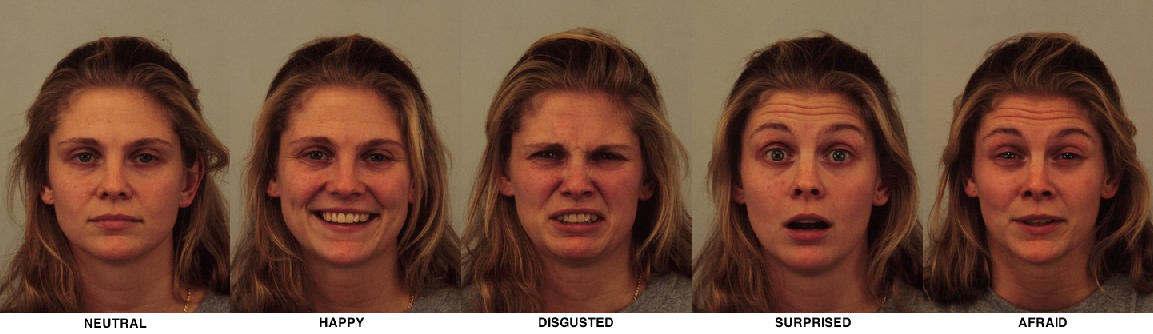
\includegraphics[scale=0.3]{figures/kdef_difference_emotions} 
\newline
\caption{Face images from the KDEF database used in the test set}
\label{kdef_difference_emotions}
\end{center} 
\end{figure}

\noindent As it can be seen in Figure~\ref{kdef_difference_emotions}, for each emotion, eyebrows are raised, eyes are widely opened, and the mouth has a distinct shape, whereas in Figure~\ref{kdef_no_difference_emotions} there are no differences as visible as in Figure~\ref{kdef_difference_emotions}. These variations of intensity might explain why the system struggles when trying to differentiate \textit{angry} and \textit{sad} emotional states.
\newline

\noindent The second group contains the 2 remaining facial expressions. The 2 facial expressions \textit{angry} and \textit{sad}, are the ones that distort the less the face. For a same subject expressing these 2 different emotions, as in Figure~\ref{kdef_no_difference_emotions}, the differences are not clearly noticeable.
\newline

\begin{figure}[!h]
\begin{center}
\noindent 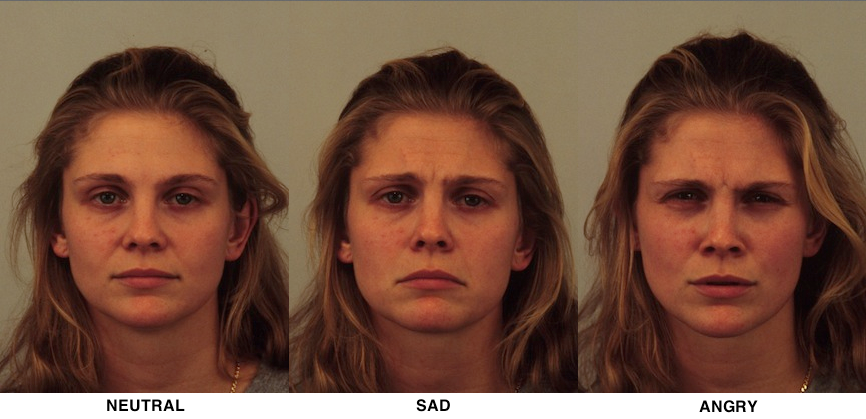
\includegraphics[scale=0.3]{figures/kdef_no_difference_emotions} 
\newline
\caption{Face images from the KDEF database used in the test set}
\label{kdef_no_difference_emotions}
\end{center} 
\end{figure}

\noindent The \textit{sad} emotion is the one that is the hardest to recognize. On 12 times, it has been well recognized only once. It is mostly taken for the \textit{neutral} state. As it can be seen in the Figure~\ref{kdef_no_difference_emotions}, there is not clear change between the \textit{neutral} state and the \textit{sad} emotion. Only the eyebrows are lightly frowned.
\newline

\noindent The \textit{angry} emotion is also hard to recognize. On 12 times, it has been well recognized only 5 times. It is mostly taken for the \textit{neutral} state and for the \textit{angry} emotion. As it can be seen in the Figure~\ref{kdef_no_difference_emotions}, there is not clear change between the \textit{neutral} state, the \textit{sad} emotion and the \textit{angry} emotion. Only the eyebrows slightly change as the eyes. The mouth is almost identical between the three face images in the Figure~\ref{kdef_no_difference_emotions}
\newline

\phantomsection
\section{Second result set}

\vspace{\baselineskip}
\noindent The second result test is processed in the same way as the first data set, the only difference being the input. Indeed, it is not performed on static images extracted from the KDEF database anymore; images used for texting are extracted from the video stream coming from the Kinect. A subject stands in front of the Kinect, his or her face is detected and extracted, then features are computed, and finally classification is performed. It runs almost in real-time, and the process outputs the name of the emotion expressed.
\newline

\subsection{With face images from the KDEF database}

\vspace{\baselineskip}
\noindent Because the results do not have a good accuracy at first sight, another method is tested. Face images from the KDEF database are given as input directly to our program. This way the data can be tested. Ten face images are randomly chosen among all the face images present in the KDEF database to be tested for each emotion. 
\newline

\noindent The model used is the one that gave the best results in the first test set: polynomial kernel with following parameters: $ D = 2 $ and $ \gamma = 0.001953125 $. Table~\ref{table_results_confusion_matrix_offline} represents the confusion matrix for this kernel and these test conditions.
\newline

\begin{table}[h]
\begin{center}
   \caption{\label{table_results_confusion_matrix_offline} Confusion matrix}
\begin{tabular}{|c|c|c|c|c|c|c|c|c|}
  \hline
   & neutral & afraid & angry & disgusted & happy & sad & surprised & accuracy \\
  \hline
  neutral & \textbf{6} & 1 & 2 & 0 & 0 & 1 & 0 & 60.00\% \\
  afraid & 0 & \textbf{4} & 0 & 3 & 0 & 3 & 0 & 40.00\% \\
  angry & 2 & 1 & \textbf{6} & 1 & 0 & 0 & 0 & 60.00\% \\
  disgusted & 0 & 1 & 0 & \textbf{7} & 1 & 1 & 0 & 70.00\% \\
  happy & 0 & 0 & 0 & 0 & \textbf{10} & 0 & 0 & 100.00\% \\
  sad & 1 & 3 & 2 & 1 & 1 & \textbf{2} & 0 & 20.00\% \\
  surprised & 0 & 0 & 0 & 0 & 0 & 0 & \textbf{10} & 100.00\%\\
  \hline
\end{tabular}
\end{center}
\end{table}

\noindent The overall accuracy rate is of $ 64.28\% $ which is lower than the one obtained in the first result set: $ 66.67\% $. The results obtained are consistent with the ones found in the first result set.
\newline

\subsection{With subjects}

\vspace{\baselineskip}
\noindent For this test set, we use face images from the JAFFE database that are placed in front of the Kinect. Ten face images has been chosen randomly from this databases for each emotion.
\newline

\noindent As for the precedent part, the model used is the polynomial kernel with the following parameters: $ D = 2 $ and $ \gamma = 0.001953125 $. Table~\ref{table_results_confusion_matrix_kinect} represents the confusion matrix for this kernel and these test conditions.
\newline

\begin{table}[h]
\begin{center}
   \caption{\label{table_results_confusion_matrix_kinect} Confusion matrix}
\begin{tabular}{|c|c|c|c|c|c|c|c|c|}
  \hline
   & neutral & afraid & angry & disgusted & happy & sad & surprised & accuracy \\
  \hline
  neutral & \textbf{6} & 0 & 0 & 0 & 0 & 4 & 0 & 60.00\% \\
  afraid & 2 & \textbf{1} & 1 & 0 & 0 & 6 & 0 & 10.00\% \\
  angry & 3 & 0 & \textbf{0} & 0 & 0 & 7 & 0 & 0.00\% \\
  disgusted & 1 & 0 & 1 & \textbf{0} & 0 & 8 & 0 & 0.00\% \\
  happy & 4 & 3 & 0 & 0 & \textbf{0} & 3 & 0 & 0.00\% \\
  sad & 4 & 0 & 0 & 0 & 0 & \textbf{5} & 1 & 50.00\% \\
  surprised & 5 & 0 & 1 & 0 & 0 & 4 & \textbf{0} & 0.00\%\\
  \hline
\end{tabular}
\end{center}
\end{table}

\noindent The overall accuracy rate is of $ 15,71\% $ which is really low compared to the precedent result that is of $ 64.28\% $  and to the one obtained in the first result set that is of $ 66.67\% $. The results obtained are consistent with the ones found in the first result set.
\newline

\phantomsection
\section{Additional results}

\vspace{\baselineskip}
\noindent One way to obtain better results with the LBP operator for this system is to add weights for each of the 42 regions of the face, as seen in Chapter~\ref{chap:lbp}. The LBP operator used in this system is already far from the basic LBP operator; it is a uniform circular LBP operator. Even though the results obtained with this operator are quite good with an accuracy of $ 66.67\% $, there is still room for improvement. Weighting the regions of the face will have an impact on the computed histogram, hence on the resulting feature vector ready for classification. \newline

\noindent The face image is divided in 42 regions ($ 7 $ rows $\times$ $ 6 $ columns), as seen in Chapter~\ref{chap:lbp}, and mentioned in \cite{GAN08}. The weights are however not applied in the same way as in \cite{GAN08}, but rather as in Figure~\ref{lbp_region_weight}. Figure~\ref{implementation_weight_example} shows an example of the division into regions of face images from the KDEF database that this system uses. Thus, border regions are less important than those containing the ROI of the face (eyes, nose, mouth). Figure~\ref{implementation_weight_example} shows an example of the division into regions of face images from the KDEF database used by this system.
\newline

\begin{figure}[!h]
\begin{center}
\noindent 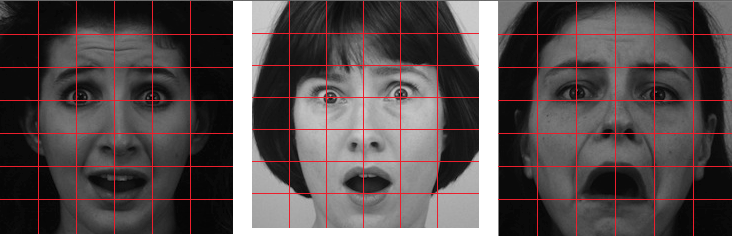
\includegraphics[scale=0.3]{figures/implementation_weight_example} 
\newline
\caption{Example of division into regions of face images from the KDEF database}
\label{implementation_weight_example}
\end{center} 
\end{figure}

\noindent Results has been obtained using the same process than for the first set result. The results with the weights applied are summed up in Table~\ref{table_results_kernels_weight}. The model has been trained with cross validation.
\newline

\begin{table}[h]
\begin{center}
   \caption{\label{table_results_kernels_weight} Results with different kernels and different parameters}
\begin{tabular}{|c|c|c|c|c|c|c|c|c|}
  \hline
    & Linear & \textbf{Poly1} & Poly2 & RBF1 & RBF2 & Sigmoid1 & Sigmoid2 \\
  \hline
  neutral & 75.00\% & 75.00\% & 91,67\% & \textbf{91,67\%} & 75.00\% & 100.00\% & 66.67\% \\
  afraid & 91,67\% & 83.33\% & 100.00\% & \textbf{100.00\%} & 83.33\% & 33.33\% & 91,67\% \\
  angry & 58.33\% & 58.33\% & 41.67\% & \textbf{66.67\%} & 58.33\% & 50.00\% & 50.00\% \\
  disgusted & 41.67\% & 58.33\% & 50.00\% & \textbf{50.00\%} & 50.00\% & 75.00\% & 41.67\% \\
  happy & 100.00\% & 100.00\% & 91.67\% & \textbf{100.00\%} & 100.00\% & 91.67\% & 91.67\% \\
  sad & 8.33\% & 8.33\% & 8.33\% & \textbf{8.33\%} & 8.33\% & 8.33\% & 8.33\% \\
  surprised & 75.00\% & 75.00\% & 75.00\% & \textbf{83.33\%} & 75.00\% & 66.67\% & 75.00\% \\
  \textbf{overall} & \textbf{64.29\%} & \textbf{65.48\%} & \textbf{{65.48\%}\%} & \textbf{{\color{red}71.42\%}} & \textbf{64.29\%} & \textbf{59.52\%} & \textbf{60.71\%} \\
  \hline
\end{tabular}
\end{center} 
\end{table}

\noindent \textit{Poly1} stands for Polynomial and has degree parameter: $ D = 2 $ and $ \gamma = 0.001953125 $
\newline
\noindent \textit{Poly2} stands for Polynomial and has degree parameter: $ D = 3 $ and $ \gamma = 0.001953125 $
\newline
\noindent \textit{RBF1} has cache and $\gamma$ parameters: $ C = 128 $ and $ \gamma = 0.0078125 $
\newline
\noindent \textit{RBF2} has cache and $\gamma$ parameters: $ C = 8192 $ and $ \gamma = 0.00048828125 $ 
\newline
\noindent \textit{Sigmoid1} has cache and $\gamma$ parameters: $ C = 128 $ and $ \gamma = 0.0078125 $
\newline
\noindent \textit{Sigmoid2} has cache and $\gamma$ parameters: $ C = 8192 $ and $ \gamma = 0.00048828125 $
\newline

\noindent A model has also been trained with same kernels and parameters but without cross-validation. Comparison has been made between the model with cross validation and the one without cross validation as it is shown in  Table~\ref{table_results_crossvalidation_weight}. Sometimes results are better with cross validation, sometimes results are better without it. The best result however is obtained with cross validation.
\newline

\begin{table}[h]
\begin{center}
   \caption{\label{table_results_crossvalidation_weight} Results with and without cross validation}
\begin{tabular}{|c|c|c|c|c|c|c|c|c|}
  \hline
    & with cross validation & without cross validation \\
  \hline
  Linear & 64.29\% & 66.67\% \\
  Poly1 & 65.48\% & 65.48\% \\
  Poly2 & 65.48\% & 65.48\% \\
  RBF1 & 71.42\% & 63.10\% \\
  RBF2 & 64.29\% & 67.86\% \\
  Sigmoid1 & 59.52\% & 60.71\% \\
  Sigmoid2 & 60.71\% & 67.86\% \\
  \hline
\end{tabular}
\end{center}
\end{table}

\noindent The best accuracy percentage is for a model trained with RBF1 kernel parameters and with cross validation, with an overall accuracy rate of$ 71.42\% $. It is obtained with a classification based on the RBF kernel and with following parameters: $ C = 128 $ and $ \gamma = 0.0078125 $. Table~\ref{table_results_confusion_matrix_weight} represents the confusion matrix for this kernel.
\newline

\begin{table}[h]
\begin{center}
   \caption{\label{table_results_confusion_matrix_weight} Confusion matrix}
\begin{tabular}{|c|c|c|c|c|c|c|c|c|}
  \hline
   & neutral & afraid & angry & disgusted & happy & sad & surprised & accuracy \\
  \hline
  neutral & \textbf{11} & 0 & 0 & 0 & 0 & 1 & 0 & 91.67\% \\
  afraid & 0 & \textbf{12} & 0 & 0 & 0 & 0 & 0 & 100.00\% \\
  angry & 2 & 0 & \textbf{8} & 0 & 1 & 1 & 0 & 66.67\% \\
  disgusted & 1 & 2 & 1 & \textbf{6} & 2 & 0 & 0 & 50.00\% \\
  happy & 0 & 0 & 0 & 0 & \textbf{12} & 0 & 0 & 100.00\% \\
  sad & 2 & 8 & 1 & 0 & 0 & \textbf{1} & 0 & 8.33\% \\
  surprised & 0 & 2 & 0 & 0 & 0 & 0 & \textbf{10} & 83.33\%\\
  \hline
\end{tabular}
\end{center}
\end{table}

\noindent As for the first test result, two emotions are hard for our system to recognize: the \textit{sad} emotion and the \textit{disgusted} emotion (see Table~\ref{table_results_accuracy_weight}). But this time this is not the \textit{angry} emotion that has bad results but the \textit{disgusted} emotion.
\newline

\begin{table}[h]
\begin{center}
   \caption{\label{table_results_accuracy_weight} Recognition accuracy of the six basic emotions and of the neutral state}
\begin{tabular}{|c|c|c|c|c|c|c|c|c|}
  \hline
   $ \leq 50\% $ & > 66.67\% \\
  \hline
  disgusted ($ 6/12 $) & afraid ($ 12/12 $) \\
  sad ($ 1/12 $) & angry ($ 8/12 $) \\
   & happy ($ 12/12 $) \\
   & surprised ($ 10/12 $) \\
   & neutral ($ 11/12 $) \\
  \hline
\end{tabular}
\end{center} 
\end{table}

\noindent Once again the \textit{sad} emotion is the one getting really bad results. However, with the weights applied to each region, better results are obtained. The percentage of accuracy is of $71.42\%$ instead of $66.67\%$ without the weights applied.
\newline

\newpage
\phantomsection
\chapter{Issues}
\label{chap:eval_issues}

\phantomsection
\section{Feature extraction}

\vspace{\baselineskip}
\noindent The feature extraction method chosen for this facial expression recognition system is the Local Binary Patterns method. As seen in chapter~\ref{chap:lbp}, there are many ways to improve the basic LBP operator. This ways can be using the circular LBP operator, using the uniform LBP operator or applying weights to each region of the face image. The basic LBP operator is quite simple but after improving it at its best, it requires more computation time but gives better result.
\newline

\noindent The LBP operator used in this system has already some improvements; it is a uniform circular LBP operator. The results obtained with this operator are quite good with an accuracy of $ 61.90\% $. But this percentage of accuracy can be improved by weighting each region of the face for example. This system has trouble recognizing some of the 7 emotions; more particularly the \textit{sad} emotion.
\newline

\noindent The Local Binary Patterns method was chosen because the LBP operator gives good results and has a discriminative power, and because the basic LBP operator is simple (and it can be improved in many ways). But there are most likely other methods that give equal results to the ones of the LBP operator or even better results. There are also certainly other methods that are more optimized than the LBP operator and that take less computation time. Even if the LBP operator seems to be a good compromise between computation time and results; other methods can be implemented to compare the performance of each algorithm with the same test conditions.
\newline

\phantomsection
\section{Real-time}

\vspace{\baselineskip}
\noindent The computation of the LBP operator takes about 1-4 seconds (depending on the computer). It was not expected that it takes so long. it was more expected to obtain a computation time on the order of milliseconds. That is why this facial expression recognition system does not really work in real-time an why it needs an interaction with the subject. With the Kinect, 30 frames are received per second. The system should take 33,3 milliseconds maximum ($ \frac{1}{30} = 0,0333 s $) so that it could work in real-time and have the time to process each frame. 
\newline

\noindent The basic LBP operator is quite simple so a system based on this feature extraction method should be able to work in real-time. Using the circular LBP operator adds some computation time; but the use of the uniform LBP allows to reduce the computation time by only considering the uniform LBP and not the non-uniform ones.
\newline

\noindent The system was adapted so that it can still work with video sequences and almost in real-time. The subject stands in front of the Kinect and express an emotion among the 6 basic ones plus the neutral one. When the subject thinks that the emotion that is expressed is good, then he can click on the interface to launch the processing with this exact face he made. Then only one frame is used, the one he chose when he clicked. This frame is processed and classified and the output given to the subject is the name of the emotion that he expressed. The output is given about 2 seconds after the subject's click.
\newline

\phantomsection
\section{Training dataset}

\vspace{\baselineskip}

\noindent bla bla bla
\newline

\stopcontents[parts]